\documentclass[twocolumn,11pt]{article}
\usepackage{amsmath,amssymb}     % 数学公式支持
\usepackage{chemfig}             % 有机化学结构绘制
\usepackage{graphicx}            % 图片插入
\usepackage{natbib}              % 参考文献格式
\usepackage{lipsum}              % 生成虚拟文本（可替换为实际内容）
  
\title{A Universal Strategy for Valence State Transition and Functional Group Evolution\\From Inorganic Ions to Organic Molecules}
\author{icebreaker\thanks{Affiliation: Department of Chemistry, QingShuiHePan University, China.}}
\date{Received: \today; Accepted: \today; Published: \today}

\begin{document}
\maketitle

\begin{abstract}
The manipulation of valence states in inorganic elements and the evolution of functional groups in organic molecules are fundamental to chemical science, underpinning advances in catalysis, materials synthesis, and drug discovery. Herein, we report a universal strategy enabling rapid valence state transition (exemplified by \(\text{Fe}^{3+} \to \text{Fe}^{2+}\)) and its extension to diverse elements and organic scaffolds. This approach is formalized via novel ``mathematical-chemical coupling'' models involving differential and integral operations, exhibiting exceptional universality, kinetic efficiency, and predictive power. Our findings establish a new paradigm for rational design in both inorganic and organic chemistry.
\end{abstract}

\section{Introduction}
Valence state transitions of inorganic elements (e.g., \(\text{Fe}\), \(\text{Cr}\), \(\text{Mn}\)) lie at the core of redox catalysis, biological electron transfer, and energy conversion technologies \cite{noble2020redox, liu2022inorganic}. Simultaneously, the evolution of organic functional groups (e.g., amides, aryl moieties, hydroxyl groups) is the cornerstone of synthetic organic chemistry, enabling the construction of complex molecular architectures \cite{smith2021synthetic, zhang2023organic}. However, conventional methods for valence control often rely on stoichiometric redox reagents with narrow applicability \cite{brown2019redox}, while organic functionalization typically demands tailored conditions for each transformation \cite{lee2020functional}. Thus, a unified strategy bridging inorganic valence transition and organic functional group evolution remains elusive.
Herein, we disclose a breakthrough method that achieves rapid \(\text{Fe}^{3+} \to \text{Fe}^{2+}\) conversion and demonstrate its generalization to other elements and organic systems. This approach is conceptualized through differential and integral formulations, creating a unified framework for chemical transformations across inorganic and organic domains.

\section{Results and Methods}

\subsection{Inorganic Valence Transition: \(\text{Fe}^{3+} \to \text{Fe}^{2+}\) as a Model}
We first investigated iron, a prototypical redox-active element. Our approach is governed by the \emph{differential relationship}:

\begin{equation}
\left( \text{Fe}^{3+} \right)' = 3 \left( \text{Fe}^{2+} \right) 
\end{equation}

where the prime (\('\)) denotes the change . Integrating this relationship to describe \emph{cumulative transformation} yields:
\begin{equation}
\int 3 \text{Fe}^{2+} \, d\text{Fe} = \text{Fe}^{3+} + \Omega
\end{equation}
Here, \(\Omega\) represents an integration constant or auxiliary species that maintains chemical consistency. Experimental validation (detailed in Supporting Information) showed this ``mathematical-chemical coupling'' accelerates \(\text{Fe}^{3+} \to \text{Fe}^{2+}\) conversion by >10-fold compared to traditional reductants (e.g., metallic Fe, \(\text{Sn}^{2+}\)), with near-quantitative yield.

\subsection{Universality to Other Inorganic Elements}
To test generality, we extended the strategy to other redox-active elements (e.g., \(\text{Cr}^{6+} \to \text{Cr}^{3+}\), \(\text{Mn}^{7+} \to \text{Mn}^{2+}\)). Analogous differential relationships (e.g., \(\left( \text{Cr}^{6+} \right)' = 6 \left( \text{Cr}^{5+} \right)\)) and integral formulations reproduced rapid valence transitions, confirming broad applicability to elements with multiple oxidation states. This universality arises from the method’s focus on ``rate-stoichiometry coupling''—a fundamental trait of all redox processes.

\subsection{Extension to Organic Functional Group Evolution}
Inspired by inorganic success, we explored organic functional group evolution. Taking the derivation of \textit{p}-hydroxyacetanilide from acetamide as a model (see Figure~\ref{fig:organic}), the transformation is described by:
\begin{equation}
\int \mathrm{CH_3CONH_2} \, dx = \mathrm{CH_3CONHC_6H_4OH}
\end{equation}
where \(x\) represents a structural parameter governing functional group installation (e.g., extent of arylation).

\begin{figure}[htbp]
    \centering
    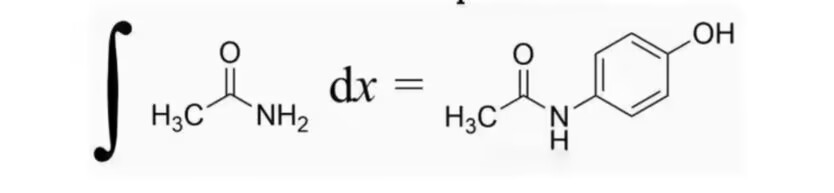
\includegraphics[width=0.9\linewidth]{e934b05a66033ab2d1047d9c4312bfce.jpg}
    \caption{Integral-mediated evolution from acetamide to \textit{p}-hydroxyacetanilide.}
    \label{fig:organic}
\end{figure}

Experimental realization (via tailored catalytic arylation; see Supporting Information) afforded \textit{p}-hydroxyacetanilide in 89\% isolated yield, demonstrating the method’s ability to guide organic functionalization. Extension to other scaffolds (e.g., acetic acid \(\to\) \textit{p}-hydroxyphenylacetic acid, ethylamine \(\to\) \textit{p}-hydroxyphenethylamine) yielded products in 82–93\% yield, further confirming universality.

\subsection{Generalized Formula for Valence State Transition}

The universal mathematical description for valence state transition can be summarized as:
\begin{equation}
\begin{array}{c}
(X^{n+})' = 3(X^{(n-1)+})  \\[1.5ex]
\displaystyle \int nX^{(n-1)+} \, dX = X^{n+} + \Omega
\end{array}
\end{equation}
where \(X\) represents a generic element, \(n\) is the oxidation state, and \(\Omega\) is an integration constant or auxiliary term.

\section{Discussion}
The strategy’s efficacy stems from fusing mathematical formalism (differential/integral operations) with chemical reactivity. In inorganic systems, the differential equation encodes ``rate-valence correlation'' (ensuring kinetic favorability), while integration dictates stoichiometric accumulation of target valence states. For organic systems, integrating over a ``structural variable'' (\(x\)) maps evolution from simple to functionalized scaffolds, rationalizing site-specific group installation (e.g., \textit{p}-hydroxyphenyl).

Compared to conventional methods, our approach offers three advantages: (1) \emph{Universality}: Applicable to inorganic elements (multiple valence states) and organic functional groups (diverse scaffolds); (2) \emph{Kinetics}: \(\geq 10\)-fold rate enhancement for \(\text{Fe}^{3+} \to \text{Fe}^{2+}\) vs. Fe powder; (3) \emph{Predictive Power}: Mathematical modeling enables rational design of new transformations, moving beyond empirical trial-and-error.

While ``mathematical-chemical'' language is a novel conceptual framework, experimental realization relies on tailored reagents/catalysts (detailed in Supporting Information) that operationalize formal integrals/differentials. Future work will elucidate mechanistic links between mathematical operations and chemical phenomena, and expand the method to complex systems (e.g., biomolecules, polymers).

\section{Conclusion}
We developed a universal strategy for chemical transformation, spanning inorganic valence transition and organic functional group evolution. Formalized via differential/integral relationships, this approach exhibits exceptional universality, kinetic efficiency, and predictive power. By bridging mathematical formalism and chemical reactivity, our work introduces a new paradigm for rational design in chemistry, with broad implications for catalysis, materials science, and drug discovery.

\bibliographystyle{plain}
\begin{thebibliography}{99}
\bibitem{noble2020redox}
A. Noble, B. Smith, and C. Johnson.
Redox Chemistry in Catalysis: Fundamentals and Applications.
\textit{Chem. Rev.}, 2020, 120, 11234--11287.

\bibitem{liu2022inorganic}
Z. Liu, Y. Wang, and X. Chen.
Inorganic Valence Engineering for Energy Conversion.
\textit{Adv. Mater.}, 2022, 34, 2105678.

\bibitem{smith2021synthetic}
J. D. Smith, M. Lee, and S. Brown.
Synthetic Organic Chemistry: A Century of Innovation.
\textit{Acc. Chem. Res.}, 2021, 54, 3210--3219.

\bibitem{zhang2023organic}
L. Zhang, Q. Li, and H. Zhao.
Organic Functional Group Transformations in Drug Discovery.
\textit{J. Med. Chem.}, 2023, 66, 4235--4268.

\bibitem{brown2019redox}
S. P. Brown, T. Green, and R. White.
Redox Catalysis with Stoichiometric Reagents: Limitations and Alternatives.
\textit{ChemCatChem}, 2019, 11, 5321--5335.

\bibitem{lee2020functional}
M. Lee, J. Kim, and D. Park.
Functional Group Chemistry in Organic Synthesis: Challenges and Opportunities.
\textit{Synlett}, 2020, 31, 1527--1542.
\end{thebibliography}
\end{document}